\begin{problem}
试结合相关协议和框架,描述一个Web Service从创建开始到被最终服务消费者调用的全过程中对服务的建模、查询和调用(服务生产和服务组合)的全过程。
\end{problem}

\begin{solution}
\begin{figure}[H]
    \vspace{-0.5em}
	\centering
	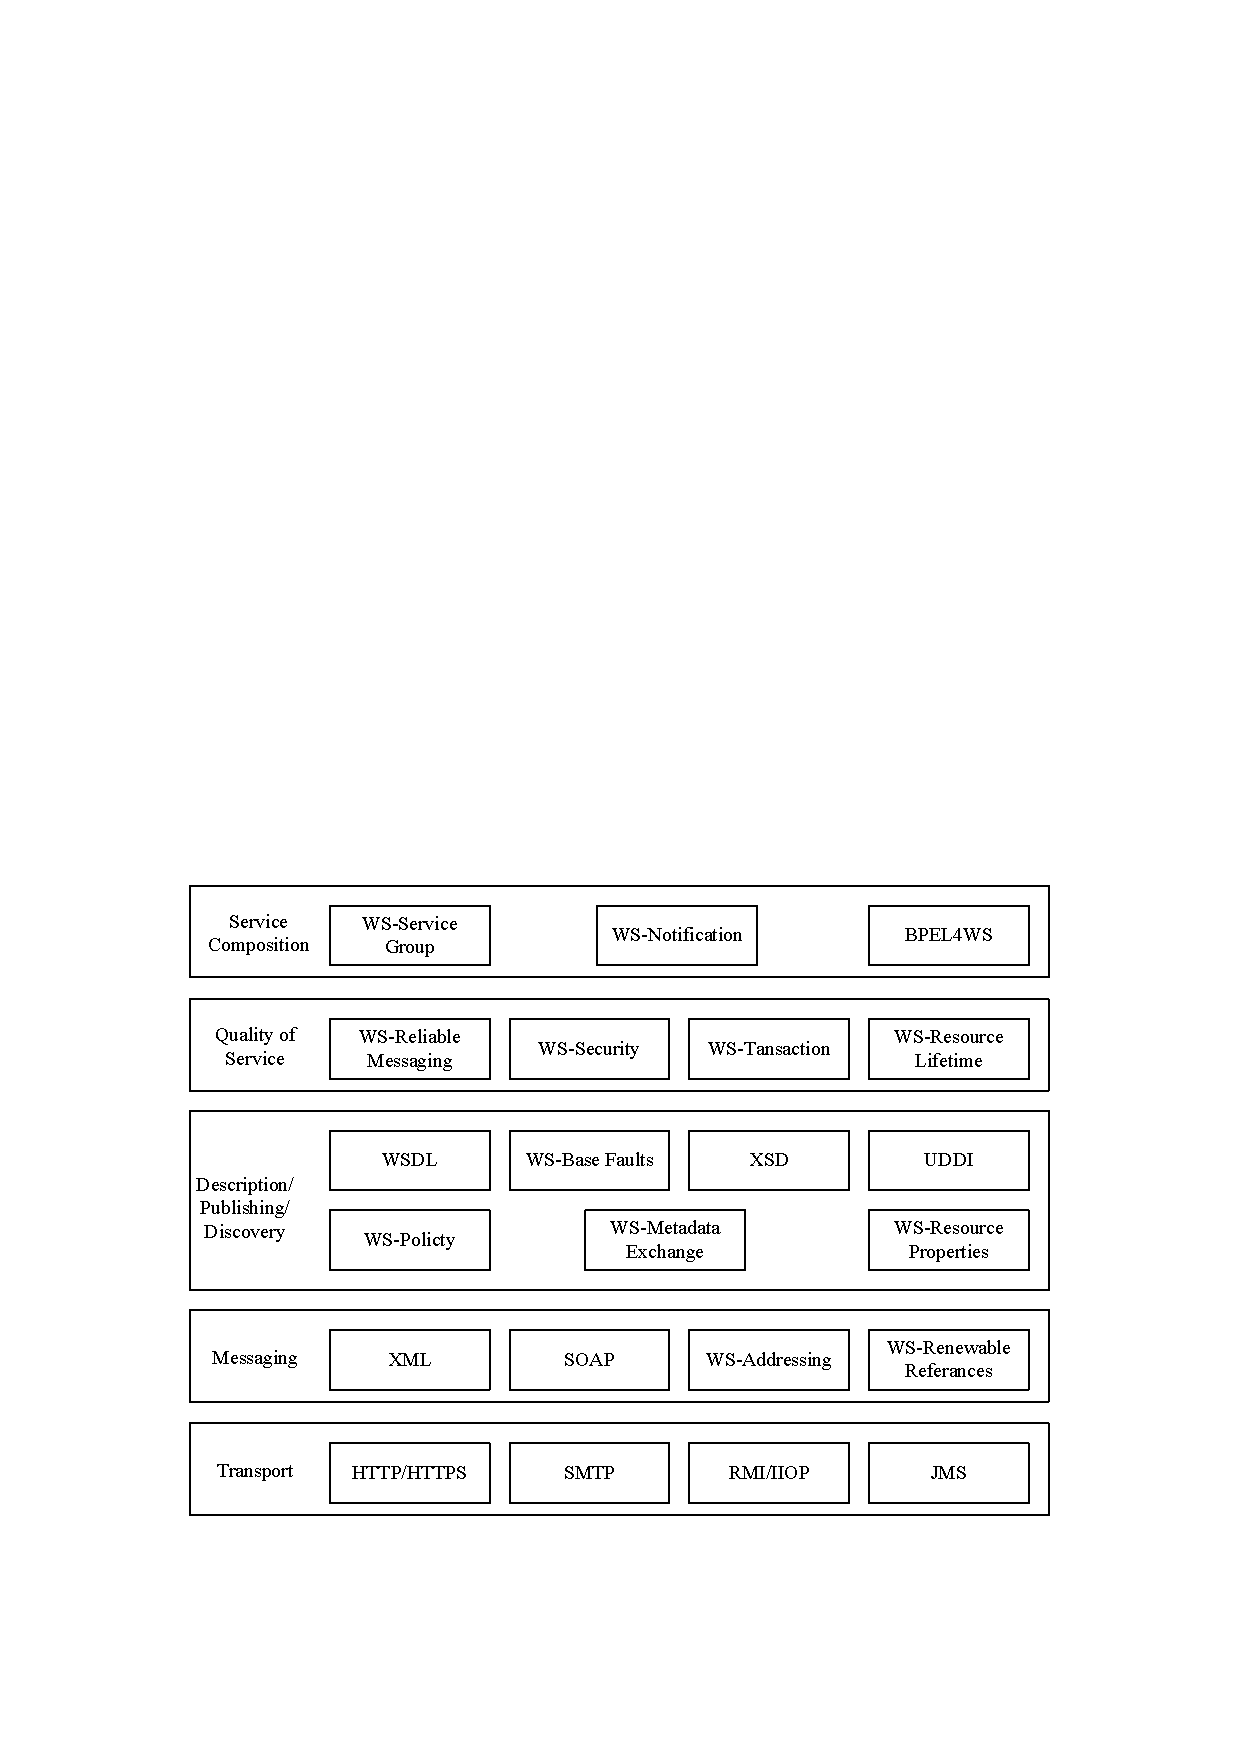
\includegraphics[width=0.75\textwidth]{Web Service过程.pdf}
    \vspace{-1em}
\end{figure}

\textbf{服务的建模}\par
服务建模是Web service 创建的第一步。在此过程中,服务提供者需要确定服务的目标,定义服务的接口和操作,并确定传输协议、消息格式和安全性要求等。在建模过程中,服务提供者可以使用不同的协议和框架,如XML,SOAP,WSDL等。
\begin{itemize}
    \item XML定义了Web服务中的消息交换格式,使用XML Schema定义不同的数据结构,引入Namespace使得XML、XML Schema中的元素和属性全球唯一旦全球共享
    \item SOAP提供了一种标准的方法,使得运行在不同平台、使用不同的技术和编程语言的应用程序可以互相进行通信,服务的发布、查找、调用,都通过SOAP传递XML消息
    \item WSDL对服务能力、服务中使用的数据结构以及传输绑定给出定义和描述;提供了一种基于XML的标准接口定义语言/服务能力定义语言,用以在服务的提供者/调用者/服务注册之间,交换必要的有关Web Service的信息
\end{itemize}

对于大多数服务,使用以上三个协议和框架可以完成建模;对于一些更为复杂的服务,如复合服务或者是带有非功能性需求的服务,还需要用到其他协议和框架完成建模。例如,BPEL定义多个服务间如何交互和合作,从而将一组现有的服务根据业务流程构建起来,实现业务服务。WS-Policy可以实现一些非功能性需求,如信息加密,权限验证等。

\textbf{服务的发布}\par
在此过程中,服务提供者将服务的描述信息发布到注册中心或其它服务目录中,以便服务消费者可以在其中查找并访问到该服务。服务描述信息应包括服务接口、操作、输入输出参数、消息格式、传输协议、安全性要求等信息。该过程可以采用UDDI或WISL方式,其中,UDDI利用分页机制,让服务得到最大可能的复用和共享范围;WSIL使用链连接结构,适用于企业既定的服务。

\textbf{服务的查询(发现)}\par
服务消费者使用服务目录(如UDDI)中的查询功能,以查找并选择适合自己的服务。在查询过程中,服务消费者可以根据服务名称、服务接口、操作、消息格式、传输协议等信息进行筛选和匹配,从而找到符合自己需求的服务。

\textbf{服务的组合}\par
在服务组合阶段,服务消费者可以将多个Web服务组合成一个较为复杂的应用程序。这个过程可以使用BPEL或WS-Coordination协议来实现。BPEL定义了服务组合的业务逻辑,WS-Coordination定义了服务协调和事务处理的规范。

\textbf{服务的调用}\par
在服务调用阶段,服务消费者可以使用客户端代理对象调用远程服务,并使用SOAP消息和XML协议与服务进行通信。服务提供者可以使用WS-Security协议来保护服务的安全性和隐私性。对于可能同时被多个消费者程序使用的服务,WS-Addressing提供了相应的机制,确保服务消费者能在实例池中找到特定的实例并与之通信。对于有状态的服务,可以利用WSRF对状态数据进行存取,进行状态管理,提高资源利用率。

服务调用过程通常包括以下步骤:
\begin{enumerate}[label=\arabic*.]
    \item 构建请求消息:服务消费者根据服务描述信息构建请求消息,并将其发送到服务提供者
    \item 消息传输:请求消息通过网络传输到服务提供者
    \item 消息处理:服务提供者接收到请求消息后,对其进行处理,生成相应消息,并将其发送回服务消费者
    \item 结果处理:服务消费者接收到相应消息后,对其进行处理,获取所需的结果并进行后续处理
\end{enumerate}

\end{solution}